%!TEX root = ../../thesis.tex
%*******************************************************************************
%****************************** Concept Chapter *********************************
%*******************************************************************************

\chapter{Solution Concept}
\label{chap:concept}
\ifpdf
    \graphicspath{{Chapters/Solution-Concept/Figs/}{Chapters/Solution-Concept/Figs/}{Chapters/Solution-Concept/Figs/}}
\else
    \graphicspath{{Chapters/Solution-Concept/Figs/}{Chapters/Solution-Concept/Figs/}}
\fi
In the previous chapter, we defined different DRs and DPs for our solution approach. 
Consequently, this chapter presents the solution concept we developed to address the \ac{dr}s and \ac{dp}s we defined in the previous chapter.
The solution concept comprises several components that work together to provide an effective and efficient solution. 
Firstly, we define the solution architecture (see section \ref{sc:section:architecture}) based on the \ac{mvc} architecture pattern. 
Secondly, we explain the \ac{ui} prototyping component (see section \ref{sc:section:prototyping}), which manages the \ac{ui} prototyping. 
Next, we present the \ac{ui} experimentation component (see section \ref{sc:section:experimentation}) responsible for managing the experimentation of the \ac{ui}, allowing us to test and evaluate different design choices and make data-driven decisions.
After that, we discuss the database components (see section \ref{sc:section:persistance}), which involve storing and retrieving data.
We then explain the deployment components (see section \ref{sc:section:deployment}) used to deploy the solution to the intended environment.
Finally, we discuss the security components (see section \ref{sc:section:security}) which ensure data security and authentication within the proposed solution.

% Consequently, in this chapter, we present the conceptual design of the solution, which outlines the system's key features, components, and functionalities. 
% This chapter bridges the gap between the solution design and the actual implementation of the solution by providing a detailed description of the solution approach.
% To visualize the system's architecture and interactions between components, we have defined software architecture (see section \ref{sc:section:architecture}) to facilitate better planning and implementation decisions.
% In section \ref{sc:section:prototyping}, we explain \ac{ui} prototyping component in detail. 
% Similarly, in section \ref{sc:section:experimentation}, we explain how to create experiments and connect participant users to experiments using our tool.
% In section \ref{sc:section:persistance}, we explain how data is stored in our database using the data models. 
% In section \ref{sc:section:deployment}, we explain the code generation and other deployment processes required to build our tool from a prototype to working software.
% Finally, in section \ref{sc:section:security}, we explain how access control for various users is managed in our security infrastructure.

% \section{Introduction}
% \label{sc:section:introduction}
% The Solution Concept chapter in software engineering provides a comprehensive understanding of the proposed solution approach. 
% This chapter bridges the gap between the solution design and the actual implementation of the solution by providing a detailed description of the solution approach. 
% It lays the groundwork for the development process, including the design decisions, and technologies used to build the software implementation. 
% Overall, in this chapter, our solution approach is based on the LEAN development cycle we defined in the previous chapter.
% To visualize the system's architecture and interactions between components, we have defined software architecture (see section \ref{sc:section:architecture}) to facilitate better planning and implementation decisions.
% In the next sections, we explain the different components we used for building our solution approach (our UI Prototyping tool). 
% In section \ref{sc:section:persistance}, we explain how data is stored in our database using the data models. 
% % In section \ref{sc:section:security}, we explain how access control for various users is managed in our security infrastructure. 
% In section \ref{sc:section:experimentation}, we explain the \ac{ui} of the tool on how to create experiments and connect participant users to experiments using our tool.
% In section \ref{sc:section:security}, we explain \ac{ui} interacts with the database. 
% Finally, in section \ref{sc:section:deployment}, we explain the code generation and other deployment processes required to build our tool from a prototype to working software.

\section{Software Architecture}
\label{sc:section:architecture}
In this section, we discuss the software architecture of our \ac{ui} prototyping tool with provisions for split and task-based usability tests. 
The software tool uses the \ac{mvc} architecture, with the main components being \textit{\ac{ui} Prototype Management} and \textit{\ac{ui} Experiment Management}. 
The models used in the architecture are the \textit{\ac{ui} Prototype} for prototyping and the \textit{\ac{ui} Experiment} for conducting the split tests. 
\begin{figure}[htbp!]
    \centering    
    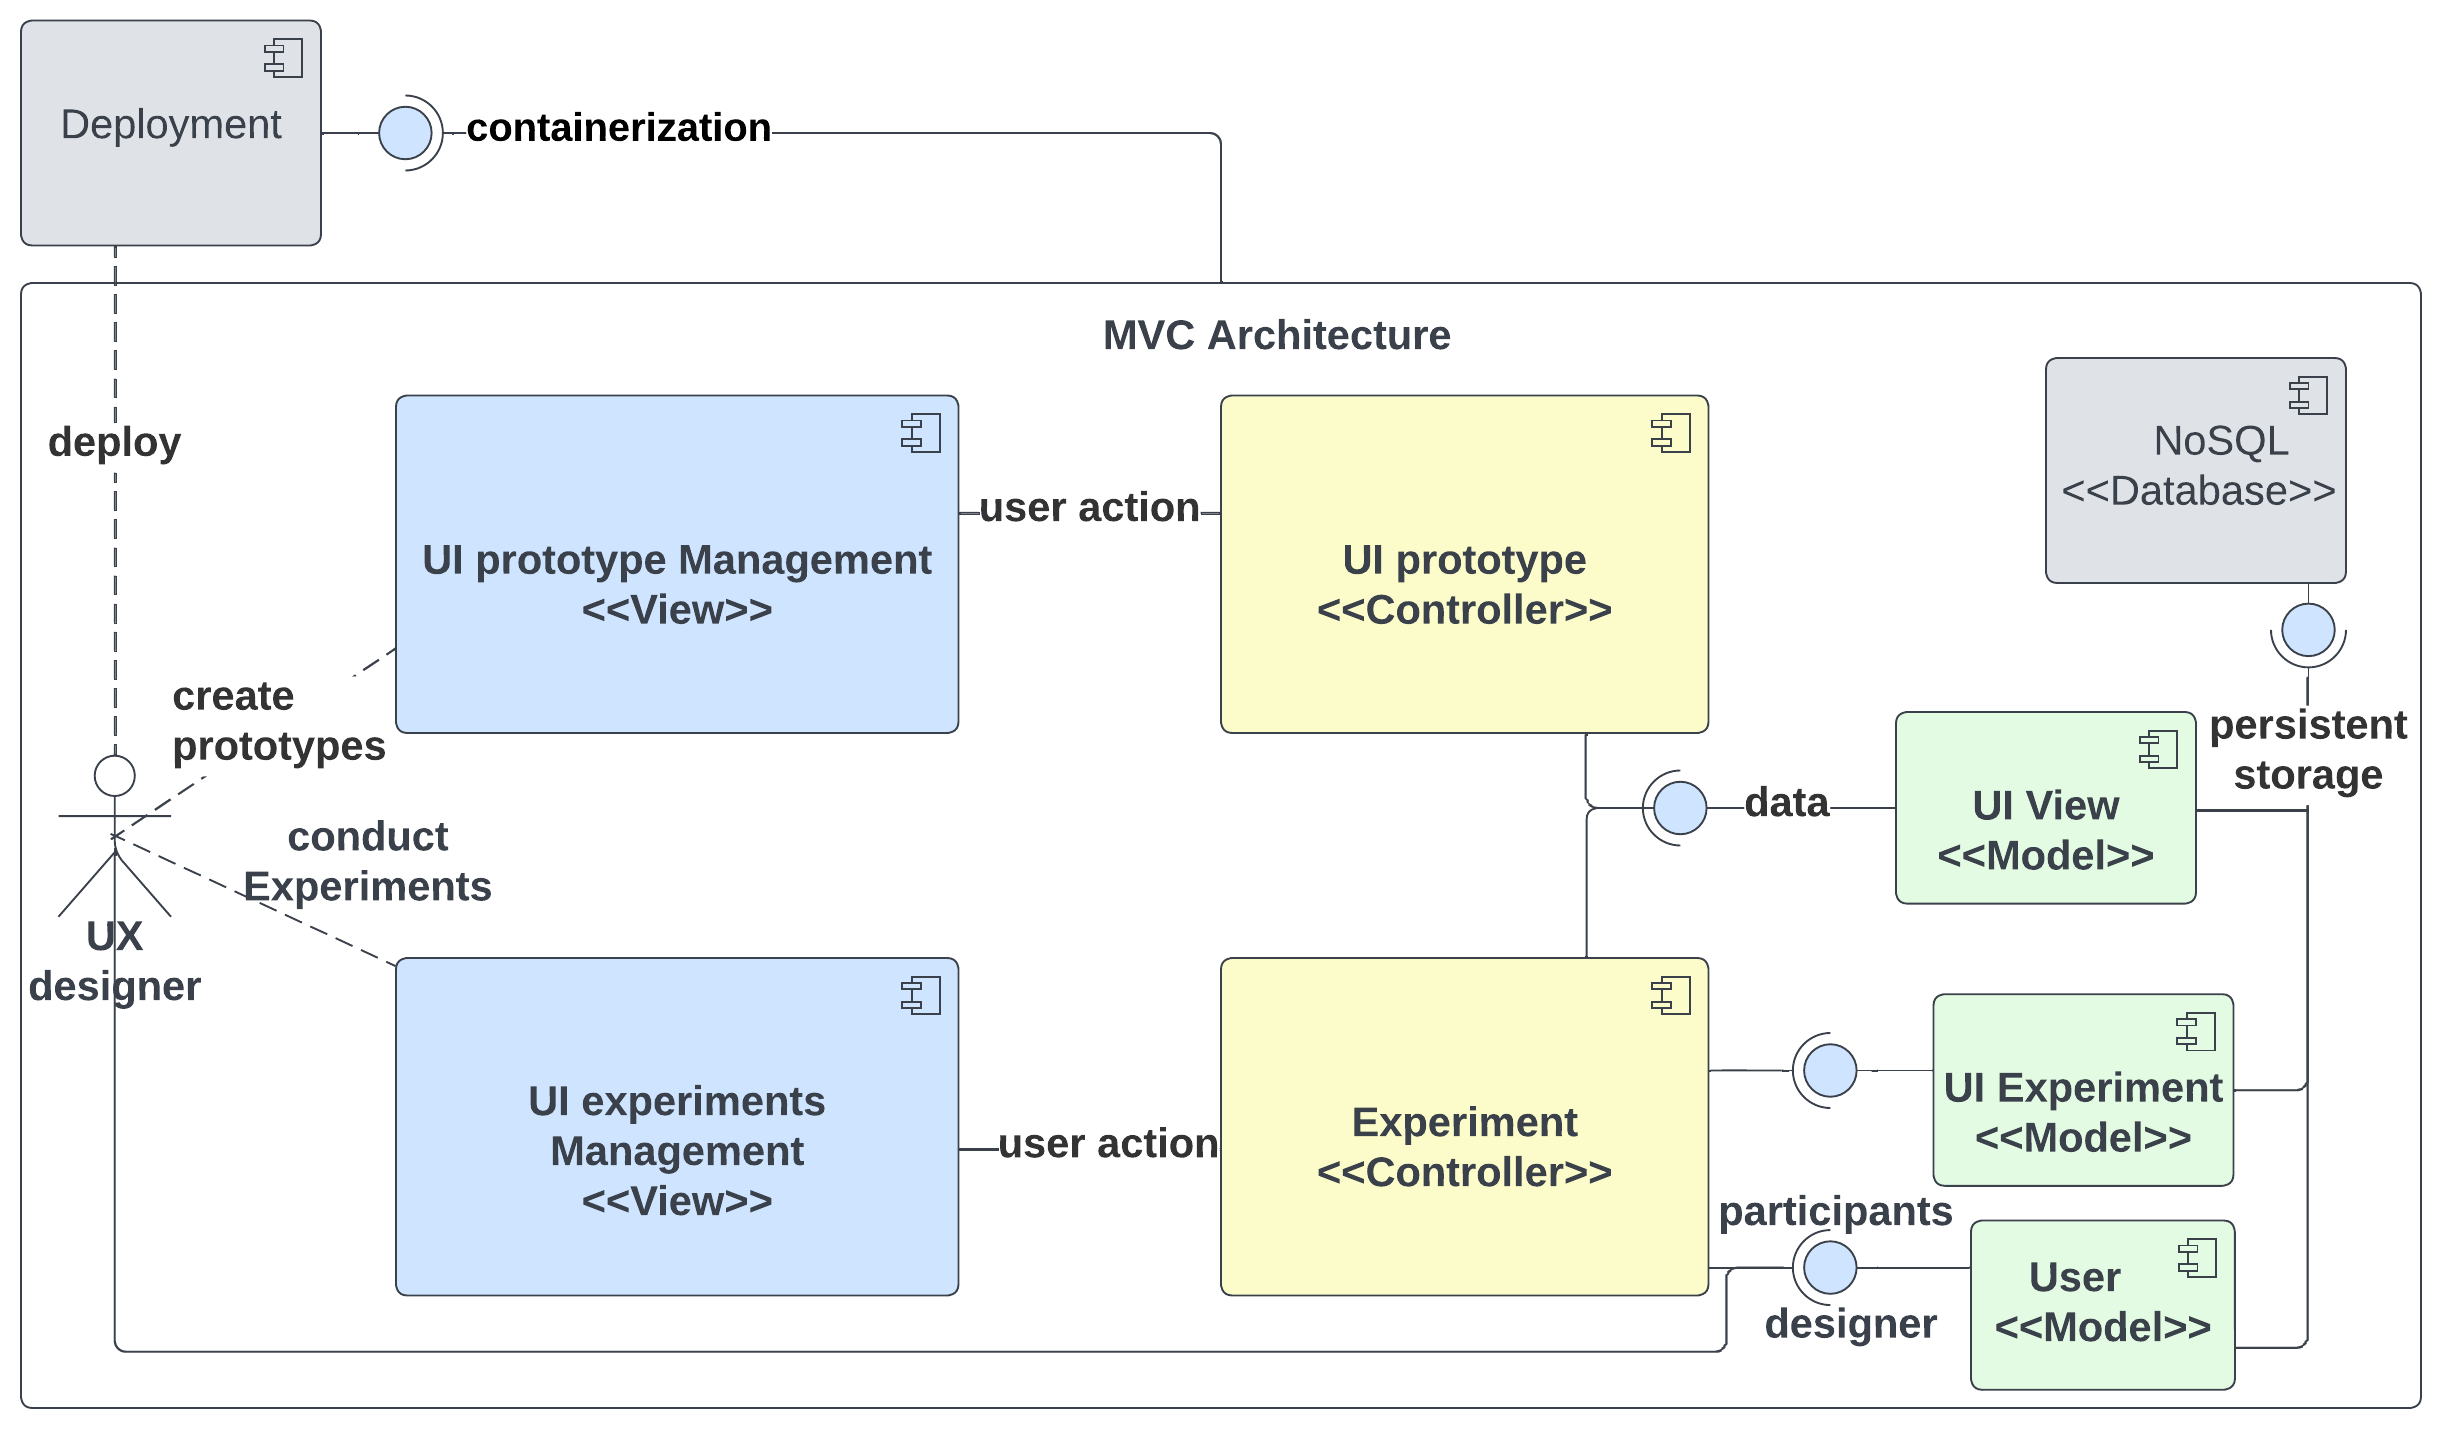
\includegraphics[width=1.0\textwidth]{MVC.png} 
    \caption[MVC Architecture of the System]{MVC Architecture of our UI Prototyping tool}
    \label{fig:sc:componentD}
\end{figure}
The diagram (see figure \ref{fig:sc:componentD}) shows the different modules and components of the \ac{ui} prototyping tool and how they interact with each other during the execution of the tool.
We chose the \ac{mvc} architecture for this tool because it separates the application logic into three interconnected components. 
The model component represents the data and the business logic of the application. 
The view component represents the application's \ac{ui}, and the controller component handles the user input and updates the model and the view. 
Separating these components allows for easier application maintenance, scalability, and modifiability.

As shown in figure \ref{fig:sc:componentD}, the \textit{UI Prototype Management} component manages the prototyping process creating different \ac{ui} screens and adding \ac{ui} elements. 
Conversely, the \textit{UI Experiment Management} component manages split tests and task-based usability tests.
Both of these components contain the controller and the view and are explained in detail in the next sections. 
These controllers handle user input and update the models and views accordingly.
The \textit{UI Prototype} model is connected to the \textit{UI Prototype Management} component, and the \textit{UI Experiment} model is connected to the \textit{UI Experiment Management} component.
These models are responsible for providing data to their respective components.
The prototyping data is stored in the \ac{db} using the \textit{\ac{ui} Prototype} model, and the \ac{ui} experimentation data is stored in the \ac{db} using the \textit{\ac{ui} Experiment} model.
At the same time, the results of the experiments also persisted in the \ac{db} using the \ac{ui} prototyping model.
Similarly, the \textit{User} model is responsible for providing the user participants for the experiments component while providing a UX designer for executing our tool.
As per the \ac{mvc} architecture, the data is then persisted into the database using a service, at the same time, the user is also allowed to do the \ac{crud} operations.  
Finally, for the database, we use a \textit{NoSQL} database that provides flexibility and scalability for applications with changing data requirements. 

The \textit{UX designers} are responsible for prototyping and creating \ac{ui} experiments and scenarios. 
They can access all the tool's features and create, edit, and delete prototypes and experiments.
Finally, for deployment, we have one component that includes all the files and dependencies required to run the application. 
This component contains the server-side code, the client-side code, and the necessary libraries and dependencies. 
The deployment component is responsible for packaging the application and deploying it to the target environment.\\\\
In summary, the software architecture for our \ac{ui} prototyping tool is designed using the \ac{mvc} architecture, with the details explained in the next sections. 
Similarly, the role of the UX designer, the user responsible for prototyping and creating user experiments and scenarios, is also described in the next section in detail.

\clearpage
\section{UI Prototype Management}
\label{sc:section:prototyping}
In our solution approach, we must have features for creating various \ac{ui} prototypes.
Therefore, using this component, we allow the \ac{ux} designers to create \ac{ui} prototypes as shown in figure \ref{fig:sc:prototyping}.
It consists of various sub-components for constructing \ac{ui} elements, data models, and analyzing results.
\begin{figure}[htbp!]
    \centering    
    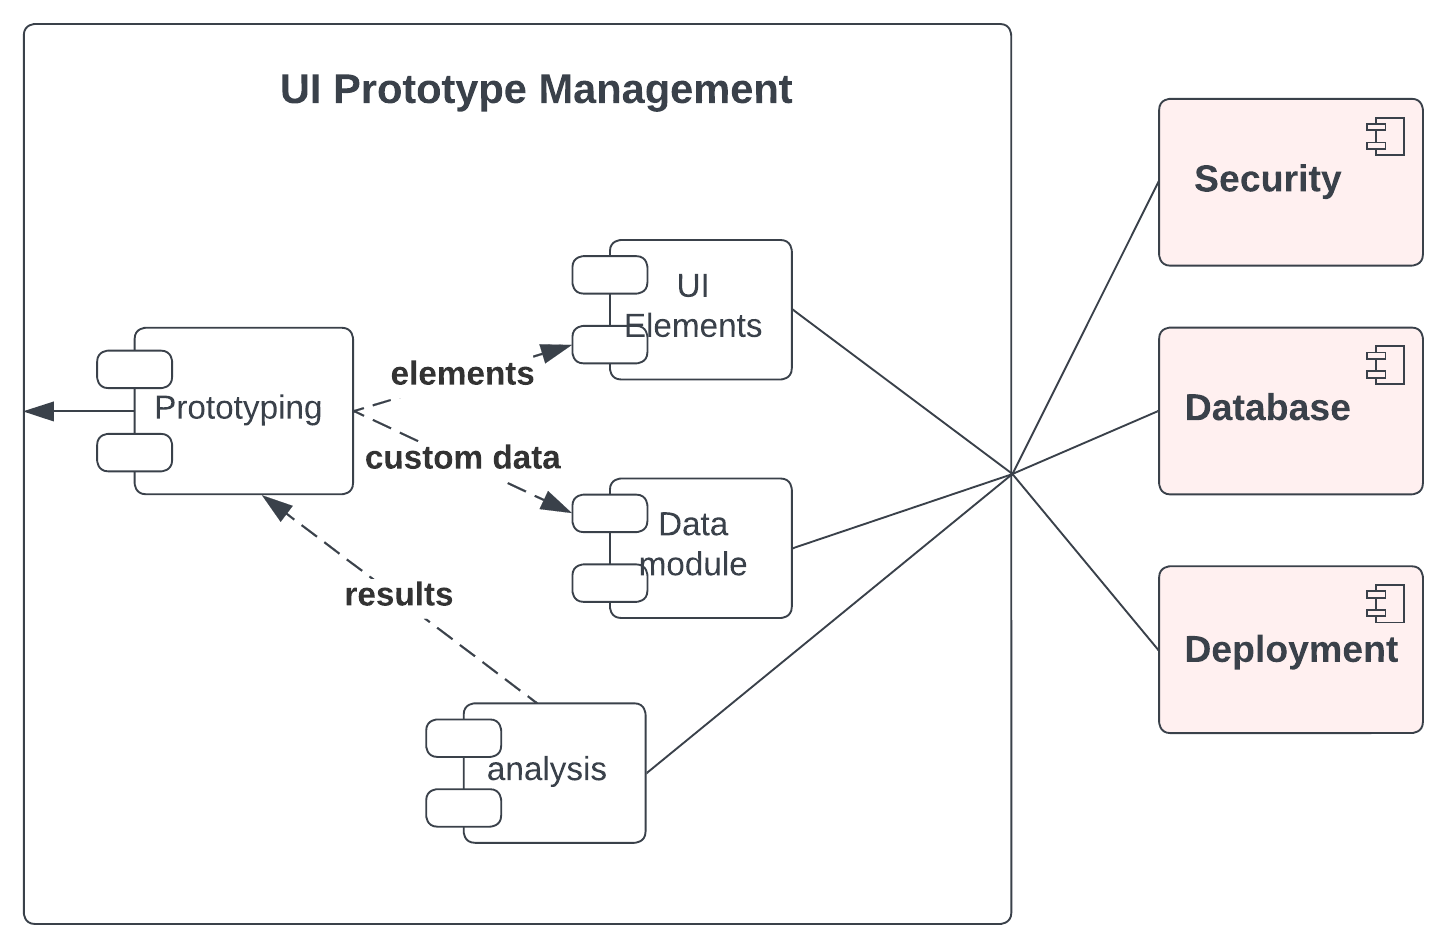
\includegraphics[width=0.9\textwidth]{UI_Prototyping.png} 
    \caption[Details of UI Prototyping Management]{Details of UI Prototyping Management connecting to a Database}
    \label{fig:sc:prototyping}
\end{figure}

\paragraph{UI Elements:}
The \textit{UI elements} component of figure \ref{fig:sc:prototyping} provides a collection of reusable and flexible UI elements that can be easily used in creating new UI prototypes.
These UI elements include buttons, input fields, dropdown menus, and many others, and are typically organized into categories for easy access and management. 
Each of our UI elements includes a range of properties that can be customized to meet the user's specific needs. 
Providing these options allows users to create prototypes that accurately represent their vision without being limited by the tool's capabilities.
Therefore, this component is crucial for quickly and efficiently creating new \ac{ui} prototypes as it eliminates the need for developers and designers to recreate the same \ac{ui} elements whenever they start a new project.

% The prototype management features a comprehensive set of UI elements designed to be reusable and easy to customize. 
% The UI Elements component represents various predefined UI elements used during the prototyping. 
% These components can be added to a screen using a simple drag-and-drop interface, allowing users to create interactive prototypes with minimal effort quickly.
% Each of our UI elements includes a range of properties that can be customized to meet the user's specific needs. 
% These properties include size, color, font, and behavior properties. 
% Providing these options allows users to create prototypes that accurately represent their vision without being limited by the tool's capabilities.
% Some UI elements we have developed include buttons, select elements, text boxes, image render, and the input element. 
% Each component is designed to be intuitive and easy to use while providing enough functionality to allow users to create complex interactions. 
\paragraph{Data Model:}
The \textit{Data Model} component of figure \ref{fig:sc:prototyping} provides a way to customize the data used in iterating the design of the \ac{ui} prototype. 
This component allows designers to define custom data models, which are then stored in a database and can be accessed and manipulated using a model.  
Similarly, these models are defined by their UI prototypes, which can be used to simulate real-world data and test the UI design in different scenarios. 
With this component, users can create data models, which are then stored in a database and can be accessed and manipulated using a model. 
This component is essential for creating realistic and comprehensive UI prototypes that more closely resemble the final product and accurately reflect the end users' needs.

% The prototype management includes a data model component allowing users to create and manage data sets for their prototypes easily. 
% With this component, users can create data models, which are then stored in a database and can be accessed and manipulated using a model.
% Creating a data model is straightforward: users import the \ac{csv} file and then create a model for the particular data set they want to use in their prototype. 
% Once the model is created, users can iterate through the data in various forms, such as a table or a grid, and visualize how the data will be displayed in their final product.
% One of the key benefits of our data model component is how easily it can be modified and updated. 
% Users can change the data directly within the model using a table, allowing them to quickly iterate on their prototypes without constantly importing new data sets. 
% This makes it easy to test different scenarios and eases the \ac{ux} designers to use the data models in the prototyping.
% Similarly, by importing real-world data sets, users can create prototypes that more closely resemble the final product, which can be valuable for testing and validation.

\paragraph{Analysis:}
The \textit{Analysis} component of figure \ref{fig:sc:prototyping} provides a way to analyze the results of the experiments conducted by the UX designer. 
This component enables users to combine and aggregate the results of qualitative and quantitative analyses.
This component allows designers to evaluate their UI prototypes' success, identify improvement areas, and make data-driven decisions about how to iterate and improve it. 
The analysis component can provide a range of data, including user feedback, metrics, and analytics, which can help designers to make informed decisions about the UI design.
It allows users to iterate quickly on their designs based on the insights gained from the analysis, ensuring that the final product is optimized.

% The prototype management includes an analysis component that enables users to combine and aggregate the results of qualitative and quantitative analyses. 
% By combining these different types of research, users can gain a more comprehensive understanding of how their prototype is performing and make data-driven decisions about how to iterate and improve it. 
% One of the key features of our analysis component is its ability to transfer the results of the winner variant back to the prototyping component. 
% It allows users to quickly iterate on their designs based on the insights gained from the analysis, ensuring that the final product is optimized for user engagement and satisfaction.\\\\
\paragraph{Prototyping:}
The \textit{Prototyping} component of figure \ref{fig:sc:prototyping} requires using all the other components mentioned above. 
The central component provides a way to create, manage, and test UI prototypes. 
By integrating the UI elements, data models, and analysis components, designers can create highly effective UI prototypes that meet the needs of the end users. 
The prototyping component typically includes features like drag-and-drop UI design tools, data uploading features, and the ability to quickly iterate and experiment with different UI design ideas.\\\\
In summary, implementing a prototyping management component simplifies UI prototyping, and helps improve the effectiveness of the UI allowing the addition of UI elements and data models and enhancing the prototype.

\clearpage
\section{UI Experimentation Management}
\label{sc:section:experimentation}
In our solution approach, we must have features for creating various \ac{ui} variants and conducting experiments of A/B testing. 
Therefore, as shown in figure \ref{fig:sc:experiments}, using this component, we allow the \ac{ux} designers to develop experiments on the UI as defined in the UI prototype.
It consists of various sub-components for constructing UI variants, assigning participants to experiments, managing participants' tasks, including qualitative questions, and collecting quantitative feedback.

\begin{figure}[htbp!]
    \centering    
    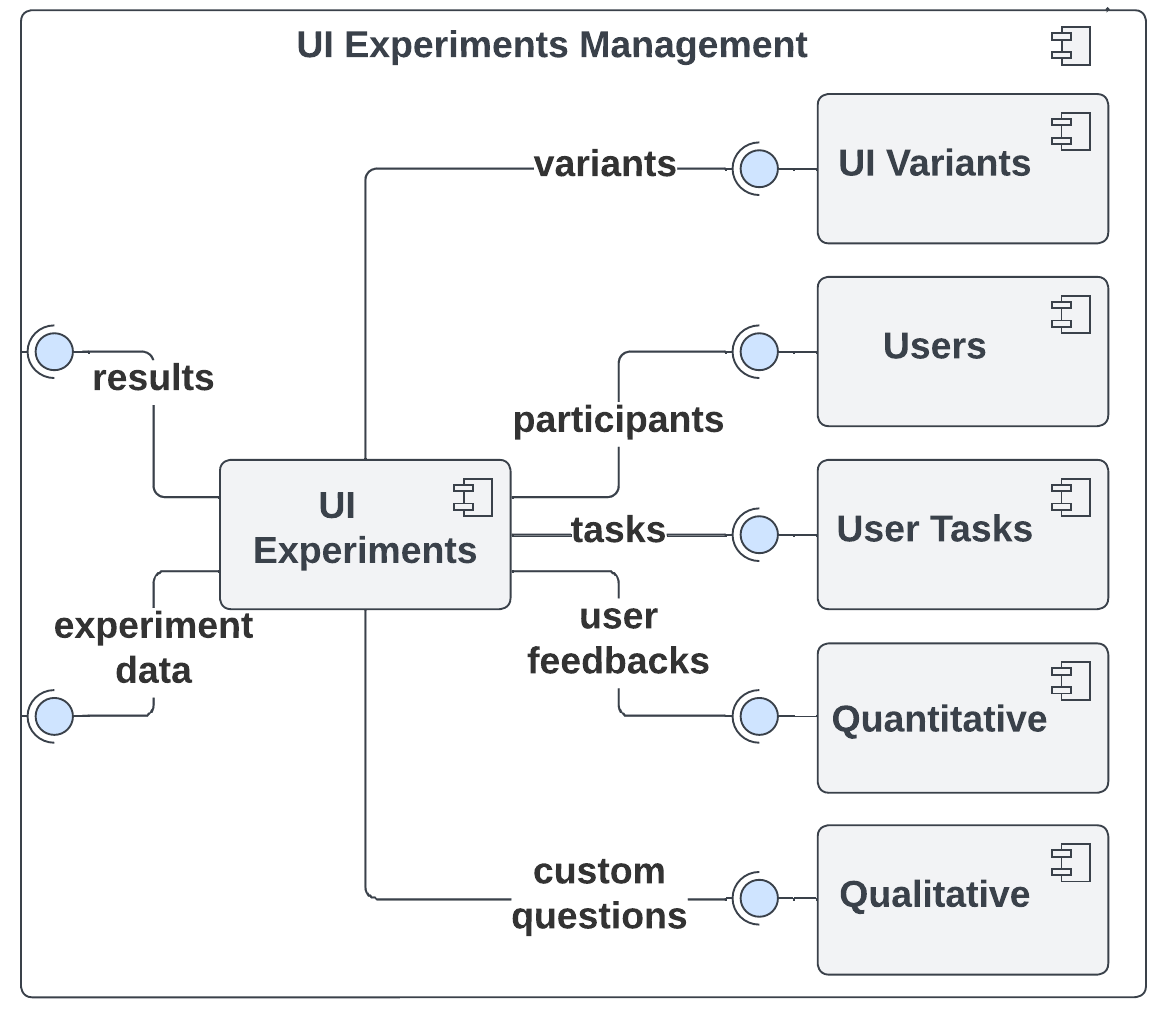
\includegraphics[width=0.9\textwidth]{UI_experiment.png} 
    \caption[Details of UI Experiment Management]{Detailed diagram of UI Experiment Management}
    \label{fig:sc:experiments}
\end{figure}

\paragraph{UI Variants:}
The \textit{UI Variants} component of figure \ref{fig:sc:experiments} allows the creation of multiple prototype variants, allowing for A/B testing and comparison between different design approaches. 
UX designers can easily customize these variants to create unique user experiences.
This component provides a range of prototype variants that UX designers can customize to suit their specific needs. 
These variants can be created and saved in the system for easy access and modification and reused across multiple experiments. 
This component ensures that designers have access to various UI variants that can be easily modified to test different hypotheses or design options.

\paragraph{Users:}
An important aspect while experimenting or A/B Testing is the users' participation. 
The \textit{Users} component provides the ability to manage user participants in UI experiments. 
It enables UX designers to create user profiles with specific characteristics and demographics and assign them to particular experiments. 
This component also provides user management functionality, including adding, removing, and editing user profiles and the ability to group users for specific experiments.

% The admin user is responsible for assigning the participants to their variants. 
% Therefore, we need to specify the percentage of participants allocated to an experiment variant during an experiment. 
% For our solution approach, we use the between-group study such that different participants test each UI variant so that each person is only exposed to a single variant. 

\paragraph{User Tasks:}
The \textit{User Tasks} component allows UX designers to create and manage tasks for participants to complete during UI experiments. These tasks can be customized to fit specific user scenarios and test different aspects of the UI design.
This component provides a task management system for participants in UI experiments. 
It allows designers to create and assign tasks to specific users and track their progress and completion. 
Tasks can be simple, such as clicking on a button or filling out a form, or more complex, such as completing a series of steps or navigating a website. 
This component ensures the UX designer measures user performance and satisfaction by assigning tasks during the \ac{ui} experimentation process.

% We need to assign them certain user tasks to get quantitative feedback from the participants. 
% It means the admin user must create certain tasks before the start of the experiment.
% Our solution approach has a \textit{Tasks} component that provides a feature for creating user tasks for every UI experiment. 
% These tasks are built and maintained in our tool by the admin user and are useful while collecting user feedback. 
% So, the participants carry out the tasks, and our tool would collect their interaction details (e.g., time taken to finish the task, the path taken by the participant, number of unsuccessful attempts). 
\paragraph{Quantitative:}
The \textit{Quantitative} component provides a mechanism for collecting user feedback on specific UI elements from tasks and experiments. 
This feedback can make data-driven decisions and inform future design iterations.
This analysis can include metrics such as time to complete a task, success rates, or user satisfaction ratings. 
The feedback can be used to evaluate the effectiveness of different design options and identify improvement areas. 
This component ensures that designers have access to quantitative data that can be used to make informed decisions during the UI experimentation process.

\paragraph{Qualitative:}
The \textit{Qualitative} component provides custom questions for the experiment and allows for gathering qualitative data from participants. 
These questions can be designed to gain insight into user perceptions, opinions, and attitudes toward the UI prototype.
These questions can be used to gather qualitative feedback from participants, such as their opinions or impressions of the design, or to elicit specific information, such as their understanding of a particular feature. 
This component ensures that designers can capture user feedback specific to the experiment.
Moreover, this component complements the quantitative part and gives users a more holistic view of how they interact with their prototype.
% The experiment management includes a qualitative component that allows users to gather participant feedback through a qualitative questionnaire. 
% This component complements the quantitative component and provides users with a more holistic view of how users interact with their prototype.
% The qualitative questionnaire can be easily added to the prototype, and users can choose from various question types, including open-ended and scale-based questions. 
% It allows users to gather rich and detailed feedback from participants about their experience with the prototype.

% The experiment management includes a quantitative component that allows users to collect data from user tasks, such as user clicks, user paths, and time taken. 
% By gathering this data, users can better understand how users interact with their prototypes and identify areas for improvement.
% Once the data has been gathered, the quantitative component calculates the mean for each metric. It provides users with an average value that they can use to compare different variations of their prototype and identify which one performs the best.
% Users can make data-driven decisions about their prototype using the mean and quickly iterate based on user feedback. 

\paragraph{UI Experiments:}
The \textit{UI Experiments} component ties the above sub-components together, providing a seamless experience for conducting UI experiments. 
Integrating all these components allows for efficient management of UI experiments and provides data analysis capabilities for informed decision-making.
This component ensures that designers have a streamlined way to manage the entire UI experimentation process, from UI variants creation to data analysis. 
It allows designers to create and execute experiments, assigning users, tasks, and prototype variants. 
Conversely, it provides an analysis of the results of the experiments, including both qualitative and quantitative data, and stores the data in a database for future use.\\\\
In summary, implementing an experiments management component simplifies the A/B testing, helps improve the effectiveness of the UI, and allows you to manage and track the different interface variations.

\clearpage
\section{Database Components}
\label{sc:section:persistance}
In our solution approach, we must have features for persisting the data in our database.
Therefore, as shown in figure \ref{fig:sc:database}, using this component, we store the data from the models from our \ac{mvc} architecture.
In the component diagram, the database components are represented by \textit{MongoDB} component and a \textit{Persistence Infrastructure}.

\begin{figure}[htbp!]
    \centering    
    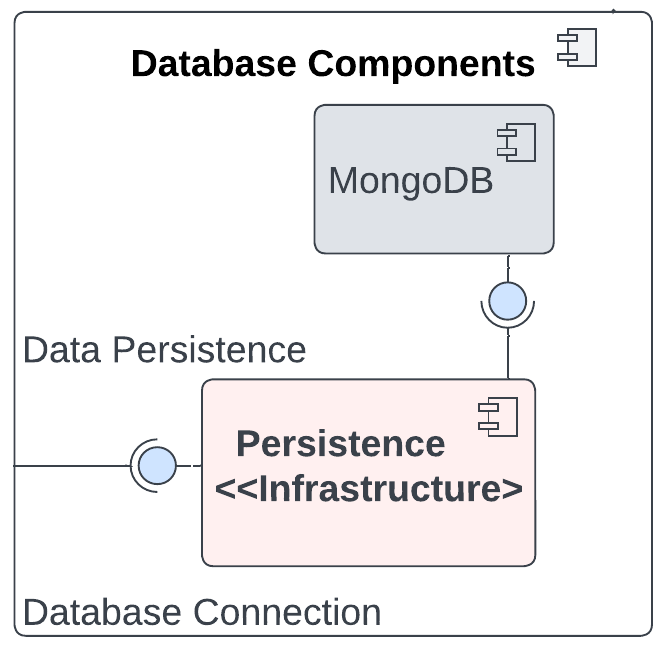
\includegraphics[width=0.65\textwidth]{Database.png} 
    \caption[Details of Database Management]{Details of Database Management}
    \label{fig:sc:database}
\end{figure}

\paragraph{Persistence Infrastructure:}
The \textit{Persistence Infrastructure} component is responsible for ensuring that the data in the database is persistent and available for future use.
Therefore, a persistence infrastructure is necessary for our software to manage a system's data storage and retrieval. 
It provides a layer of abstraction between the application and the database, which enables us to easily switch between different database types and optimize the data storage for our needs. 
The component ensures data consistency and reliability, even during system failures or errors. 
It provides a set of APIs and tools for data access and manipulation, including \ac{crud} operations in the database.

\clearpage
\paragraph{MongoDB:}
\textit{MongoDB} component represents the database components.
It is a NoSQL database that stores data in collections instead of tables, allowing for flexible and scalable data storage. 
In our \ac{mvc} architecture, MongoDB provides the application's database connection, allowing it to store and retrieve data. 
MongoDB is also known for its ability to handle large amounts of unstructured data, making it a popular choice for modern web applications.\\\\
In summary, when implementing a persistence infrastructure for a non-relational database like MongoDB, we developed the structure and functionality of the database and designed the persistence layer accordingly. 
Therefore, the system can store and retrieve data in an efficient, scalable, and reliable way.

% \paragraph{Data Persistance}
% After setting up the necessary drivers or libraries to connect to the MongoDB instance from the components in the system, we define the necessary CRUD (create, read, update, delete) operations for the data models.
% These include methods for inserting, updating, deleting, and retrieving data from the database. 
% It also provides the necessary validation and error handling for the data models and CRUD operations.

\clearpage
\section{Deployment Components}
\label{sc:section:deployment}
A deployment infrastructure is necessary for ensuring that the system is deployed and running in a secure, scalable, and reliable way. 
A deployment infrastructure is responsible for managing the deployment of components, ensuring that they are running on the appropriate servers or cloud-based environments, and monitoring their performance.
We use a no-code approach and microservice architecture to simplify deployment infrastructure implementation. 
It allows for the creation of deployment pipelines and automates many of the processes involved in deploying components.

\begin{figure}[htbp!]
    \centering    
    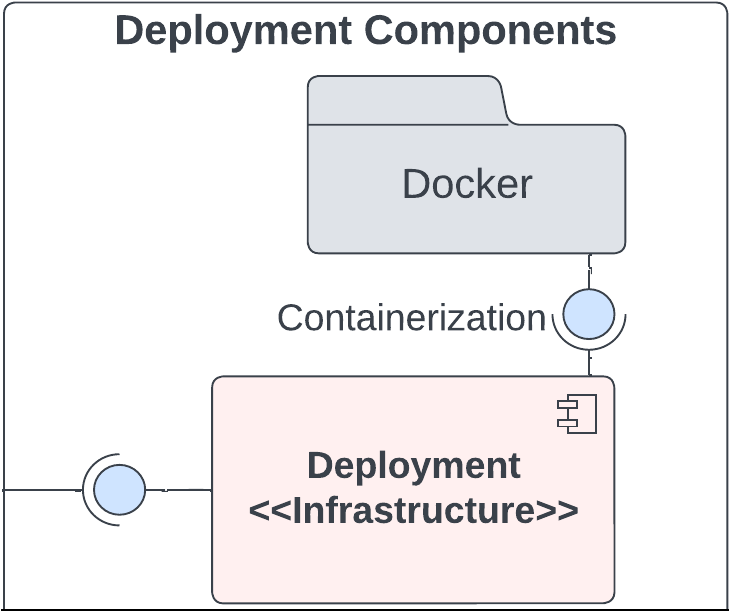
\includegraphics[width=0.6\textwidth]{Deployment.png} 
    \caption[Details of Deployment Components]{Details of Deployment Components}
    \label{fig:sc:deployment}
\end{figure}

\paragraph{Deployment Infrastructure:}
We use a no-code approach using code generation to simplify the implementation of our deployment infrastructure by automating many of the tasks involved in deploying the system.
So, we define a set of rules and templates for automatic code generation and generate some reusable components as defined by the UI prototyping management. 
These components' implementation uses templates containing its code (e.g., for a button element defined in the UI prototype, a template is generated containing all its properties and logic).
Then, the code generator takes input data, including configuration files, database schemas, and models of system components and their interactions. 
Finally, the code will be generated using the templates and rules defined in the previous steps, and we will containerize the generated code. 

\paragraph{Docker:}
Containerization plays an even more important role in using a microservice architecture. 
It must support the deployment of many independent microservices that may be deployed across multiple servers or databases.
From our component diagram, we first identify the system's microservices and their dependencies, such as database components, UI prototyping management, and UI experimentation management. 
It helps determine how the microservices should be deployed and how they should communicate.
Next, we create Docker images for each microservice and its dependencies.
Then, we define docker-compose files\footnote{A Docker Compose file is a YAML file that specifies the microservices, their dependencies, and how they should be deployed and connected.} in yaml\footnote{Website for YAML format: \url{https://www.redhat.com/en/topics/automation/what-is-yaml}} (see Appendix \ref{appendix:one:installation}) that describe how the docker containers should be deployed and connected.
Finally, we build the \textit{docker images} and deploy them as \textit{docker containers}. \\\\
In summary, implementing a deployment infrastructure for a microservice architecture can simplify the deployment and management of microservices, making it easier to build and maintain complex systems.

\clearpage
\section{Security Components}
\label{sc:section:security}
Security infrastructure is essential to protect the system from unauthorized access and attacks. 
By implementing security measures, such as access control, we limit access to sensitive information and functions to only authorized users.
Similarly, authentication is one of the fundamental security mechanisms used to verify the identity of users.
Our security infrastructure, therefore, provides access control and some authentication mechanisms (see figure \ref{fig:sc:security}).

\begin{figure}[htbp!]
    \centering    
    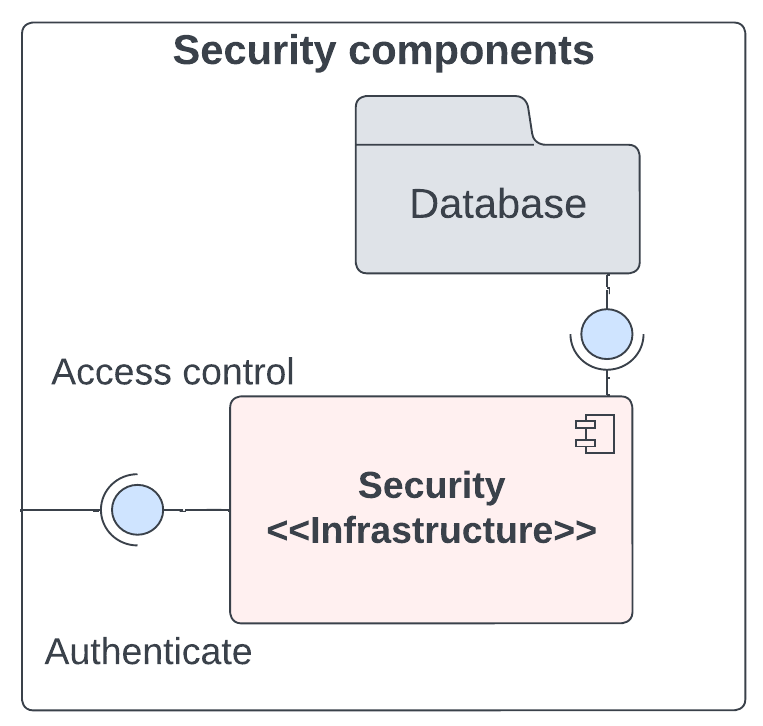
\includegraphics[width=0.6\textwidth]{Security.png} 
    \caption[Details of Security Components]{Details of Security Components}
    \label{fig:sc:security}
\end{figure}

\paragraph{Security Infrastructure:}
The \textit{Security Infrastructure} provides access control and authentication mechanisms.
Access control involves defining policies and rules determining who can access resources under what circumstances.
Therefore we implement access control mechanisms using role-based access control (RBAC) and then allowing or denying access based on those roles or groups.
So, we first identify the roles or groups requiring system access, including participants, \ac{ux} designers, and other users\footnote{This may include different stakeholders like product managers, developers, etc.}. 
Then we define the access rights (e.g., the UI prototyping management should only be accessible to the \ac{ux} deginers).
Finally, we implement a mechanism that checks the user roles and then accesses the data or services accordingly. 

Next, authentication involves verifying the identity of users and ensuring that they have the appropriate permissions to access the system.
We provide an authentication mechanism using a password and username. 
It ensures that only authorized users can access our tool.
Moreover, we define some validators for password strength to make sure the passwords are strong.\\\\
In summary, implementing a security infrastructure providing access control and authentication mechanisms for our tool can help prevent unauthorized access and protect sensitive data from being compromised.

\clearpage